\documentclass[presentation]{beamer}
\usetheme{Antibes}
\usecolortheme{dolphin}
%\usepackage{amsmath}
\usepackage{amsthm}
\usepackage{amssymb}
\usepackage{graphicx}
\usepackage{fullpage}
\usepackage{enumerate}
\usepackage{array}
\usepackage{multicol}
%\usepackage{youngtab}
\usepackage{float}

\usepackage[utf8x]{inputenc}
\usepackage{default}
\usepackage{amssymb,amsfonts,amsbsy,amsmath}
%\usepackage{tkz-graph}
\usepackage{amsmath}
\usepackage{graphicx}

\newcommand{\mycirc}[1]
{\textcircled{\raisebox{-.8pt}{#1}}}

\newcommand{\mytwo}[2]
{\raisebox{1.1pt}{\scriptsize #1} \hspace{1pt} \raisebox{-1.1pt}{\scriptsize #2}}


%% Some useful operatorname declarations for nice texing.
\newcommand{\Aut}{\operatorname{Aut}}
\newcommand{\Inn}{\operatorname{Inn}}
\newcommand{\Ker}{\operatorname{Ker}}
\newcommand{\Stab}{\operatorname{Stab}}
\newcommand{\orb}[1]{\mathcal{O}_#1}
\newcommand{\lcm}{\operatorname{lcm}}
\newcommand{\U}{\operatorname U}
\newcommand{\cl}{\operatorname {cl}}

%% Stuff from King's .tex files
\newcommand{\untab}{\noindent \!\!\!\!\!\!\!\!\!}
\newcommand{\lra}{\longrightarrow}
\newcommand{\mb}[1]{\mathbf{#1}}
\newcommand{\gap}{\vspace{0.1in}}
\DeclareMathOperator{\grad}{grad}
\DeclareMathOperator{\curl}{curl}
\DeclareMathOperator{\GL}{GL}
\newcommand{\myline}
{\vspace{.2in}
  \begin{center}
    \rule{5in}{.7pt}
  \end{center}
  \vspace{.2in}}

\usepackage{parskip}

\setlength{\parindent}{2ex}
\setlength{\parskip}{2ex plus 1ex minus 1ex}
%%% Good old "not sure if equal"
\newcommand{\qe}{\stackrel{?}{=}}

%% Some quickies for the big groups
\newcommand{\Q}{\mathbb Q}
\newcommand{\F}{\mathbb F}
\newcommand{\Qp}{\mathbb Q^+}
\newcommand{\Qn}{\mathbb Q^-}
\newcommand{\Qs}{\mathbb Q^*}
\newcommand{\R}{\mathbb R}
\newcommand{\Rp}{\mathbb R^+}
\newcommand{\Rn}{\mathbb R^-}
\newcommand{\Rs}{\mathbb R^*}
\newcommand{\Z}{\mathbb Z}
%\newcommand{\N}{\mathbb N}
%\newcommand{\C}{\mathbb C}

\newcommand{\Af}{\mathbb A}
\newcommand{\PP}{\mathbb P}

\newcommand{\GF}{\mathbb GF}

\newcommand{\gl}{\mathfrak g}
\newcommand{\bl}{\mathfrak b}
\newcommand{\tl}{\mathfrak t}
\newcommand{\pl}{\mathfrak p}
\newcommand{\nl}{\mathfrak n}

\DeclareMathOperator{\sh}{sh}

\newcommand{\Orb}{\mathcal O}
\newcommand{\Var}{\mathcal V}

\newcommand{\Irr}{\operatorname{Irr}}

\newcommand{\Brak}{[\cdot,\cdot]}

\newcommand{\NWN}{\nl \cap {^w\nl}}
\newcommand{\closeGNWN}{\overline{G \cdot (\NWN)}}

\newcommand{\N}{\mathbb N}
\newcommand{\C}{\mathbb C}

\newcommand{\GLn}{GL_n(\C)}
\newcommand{\gln}{\mathfrak {gl}_n}

\newcommand{\rank}{\operatorname{Rank}}

\newcommand{\bracket}{[\cdot, \cdot]}

\newcommand{\LRGfxSymArrowTwo}[2]{%
  \raisebox{1.3cm}{ \centering \parbox{.6cm}{ \centering%
    {\scriptsize $#1$}\\[-.23cm]$\longrightarrow$\\[-.3cm]%
    $\longleftarrow$\\[-.23cm] {\scriptsize $#2$}%
  } }%
}

% \newcommand{\LRGfxSymArrowTwo}[2]{
%   \raisebox{1.3cm}{
%     \begin{tabular}{c}
%       \centering%
%       {\scriptsize $#1$}\\[-.23cm]
%       $\longrightarrow$\\[-.3cm]%
%       $\longleftarrow$\\[-.23cm]
%       {\scriptsize $#2$}%
%     \end{tabular}
%   }
% }

\newcommand{\LRGfxSymArrow}[1]{
  \LRGfxSymArrowTwo{#1}{#1}
}
%% Good old "not sure if equal"
\newcommand{\qe}{\stackrel{?}{=}}

\makeatletter
\DeclareRobustCommand{\em}{%
  \@nomath\em \if b\expandafter\@car\f@series\@nil
  \normalfont \else \bfseries \fi}
\makeatother
\renewcommand<>{\emph}[1]{{\em #1}}

%% Some quickies for the big groups
\newcommand{\Q}{\mathbb Q}
\newcommand{\F}{\mathbb F}
\newcommand{\Qp}{\mathbb Q^+}
\newcommand{\Qn}{\mathbb Q^-}
\newcommand{\Qs}{\mathbb Q^*}
\newcommand{\R}{\mathbb R}
\newcommand{\Rp}{\mathbb R^+}
\newcommand{\Rn}{\mathbb R^-}
\newcommand{\Rs}{\mathbb R^*}
\newcommand{\Z}{\mathbb Z}
%\newcommand{\N}{\mathbb N}
%\newcommand{\C}{\mathbb C}

\newcommand{\Af}{\mathbb A}
\newcommand{\PP}{\mathbb P}

\newcommand{\GF}{\mathbb GF}

\newcommand{\gl}{\mathfrak g}
\newcommand{\bl}{\mathfrak b}
\newcommand{\tl}{\mathfrak t}
\newcommand{\pl}{\mathfrak p}
\newcommand{\nl}{\mathfrak n}

\DeclareMathOperator{\sh}{sh}

\newcommand{\Orb}{\mathcal O}
\newcommand{\Var}{\mathcal V}

\newcommand{\Irr}{\operatorname{Irr}}

\newcommand{\Brak}{[\cdot,\cdot]}

\newcommand{\NWN}{\nl \cap {^w\nl}}
\newcommand{\closeGNWN}{\overline{G \cdot (\NWN)}}

\newcommand{\N}{\mathbb N}
\newcommand{\C}{\mathbb C}

\newcommand{\GLn}{GL_n(\C)}
\newcommand{\gln}{\mathfrak {gl}_n}

\newcommand{\rank}{\operatorname{Rank}}

%\usepackage{svg}
\usepackage{graphicx}
%\usepackage{mathrsfs}
%\usepackage{setspace}
%\usepackage{showkeys}
\usepackage{amsmath}
\usepackage{hyperref}
\usepackage{tikz}
\usepackage{pgfplots}
\usepackage{pgfplotstable}
\usepackage{array}
\pgfplotsset{compat=1.5.1}
\usetikzlibrary{positioning,arrows,knots,calc,decorations.markings}

\definecolor{beamerblue}{RGB}{234,233,243}
\definecolor{beamerviolet}{RGB}{47,23,132}
\definecolor{beamerliteviolet}{RGB}{137,127,207}

\tikzset{onslide/.code args={<#1>#2}{%
  \only<#1>{\pgfkeysalso{#2}} % \pgfkeysalso doesn't change the path
}}
\tikzset{temporal/.code args={<#1>#2#3#4}{%
  \temporal<#1>{\pgfkeysalso{#2}}{\pgfkeysalso{#3}}{\pgfkeysalso{#4}} % \pgfkeysalso doesn't change the path
}}

\tikzset{
  invisible/.style={opacity=0},
  visible on/.style={alt={#1{}{invisible}}},
  alt/.code args={<#1>#2#3}{%
    \alt<#1>{\pgfkeysalso{#2}}{\pgfkeysalso{#3}} % \pgfkeysalso doesn't change the path
  },
}

\newcommand{\Uhyp}{\mathcal U} \newcommand{\Vhyp}{\mathcal V}
\newcommand{\Rhyp}{\mathcal R}


\title{Random Planar Diagrams}
\institute[UGA]{University of Georgia}
\author[Chapman]{Harrison Chapman}
\date{AMS Western Spring Sectionals 2015 (UNLV) -- April 18, 2015}

%\allowdisplaybreaks
%\usepackage[bookmarks,bookmarksopen,bookmarksdepth=4]{hyperref}

\newcommand{\so}[1]{\mathfrak {so}(#1)}

%\newtheorem{theorem}{Theorem}[section]
%\newtheorem{lemma}[theorem]{Lemma}
%\newtheorem{definition}[theorem]{Definition}
\newtheorem{proposition}[theorem]{Proposition}
%\newtheorem{corollary}[theorem]{Corollary}

%\renewcommand*\showkeyslabelformat[1]{\normalfont\tiny\ttfamily(#1)}

\graphicspath{{../../figs/}{figs/}}

\let\oldemptyset\emptyset
\let\emptyset\varnothing

\DeclareMathOperator{\Arm}{Arm}
\DeclareMathOperator{\Pol}{Pol}
\DeclareMathOperator{\UP}{UP}
\DeclareMathOperator{\VP}{VP}
\DeclareMathOperator{\APol}{APol}
\DeclareMathOperator{\Diff}{Diff}
\DeclareMathOperator{\Sympl}{Sympl}
\DeclareMathOperator{\ev}{ev}
\DeclareMathOperator{\Ad}{Ad}
\DeclareMathOperator{\crit}{crit}
\DeclareMathOperator{\ind}{ind}
\DeclareMathOperator{\intr}{int}
\DeclareMathOperator{\Hom}{Hom}
\DeclareMathOperator{\Ext}{Ext}
\DeclareMathOperator{\codim}{codim}
\DeclareMathOperator{\Ann}{Ann}
\DeclareMathOperator{\im}{Im}
\DeclareMathOperator{\Int}{int}

\begin{document}

\newcommand{\Oh}[1]{\mathcal O (#1)}
\newcommand{\g}{\mathfrak g}
\newcommand{\ShSet}{\mathcal S}
\newcommand{\LnSet}{\mathcal L}
\newcommand{\sr}{/\!\!/}

\begin{frame}
\titlepage

\end{frame}

\section{Random Planar Diagrams}
\label{sec:randompd}
\newcommand{\Salpha}[1]{S^2_{\alpha_{#1}}}

\subsection{Definition}

\begin{frame}
  \frametitle{Link shadows}
  \begin{definition}
    A \emph{link shadow} with $n$ vertices is an equivalence class
    of connected 4-regular embedded planar multigraphs with $n$
    vertices up to \emph{shadow isomorphism}.
  \end{definition}

  Two shadows are shadow-isomorphic if they are graph-isomorphic
  under a map which preserves the counterclockwise order of edges
  around each vertex.

\end{frame}
  
\begin{frame}
  \frametitle{Examples of link shadows}
  
  The following are four examples of link shadows.

  \begin{center}
    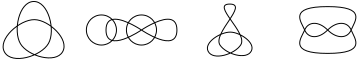
\includegraphics[width=4in]{linkshadow.pdf}
  \end{center}

  The leftmost and rightmost shadows are actually isomorphic shadows;
  they differ in choice of exterior face.
\end{frame}

\begin{frame}
  \frametitle{Components and knot shadows}
  Two edges of a link shadow are said to belong to the same
  \emph{component} if they meet at opposite ends of some vertex.

  \begin{definition}
    A link shadow is a \emph{knot shadow} if all edges in the shadow
    belong to the same component.
  \end{definition}

  An \emph{orientation} on a component is a choice of directions on
  edges in the component such that opposite edges meeting at a
  vertex point head-to-tail.
\end{frame}

\begin{frame}
  \frametitle{Link shadows and curves}
  It is well understood that

  \begin{proposition}
    The (finite) set of knot shadows with $n$ vertices is in bijection
    with the set of generic immersions of $S^1$ into $S^2$ up to
    orientation-preserving diffeomorphisms of the sphere.
  \end{proposition}
\end{frame}

\begin{frame}
  \frametitle{Diagrams}
  \begin{definition}
    A \emph{link diagram} (or planar diagram) is a link shadow where
    each component is oriented and each vertex is decorated with
    over-under information for opposite edge pairs meeting at the
    vertex, modulo \emph{diagram isotopy}.
  \end{definition}

  Two diagrams are diagram isotopic if they are shadow isomorphic
  under a map which preserves orientation of components and over-under
  information at the vertices.

  The decorated vertices are called \emph{crossings}.

  If the underlying shadow of a link diagram is a knot shadow, then
  we call it a \emph{knot diagram}.
\end{frame}

\begin{frame}
  \frametitle{Random diagrams}
  \begin{definition}
    In the \emph{random diagram model} of random knotting, a
    $n$-crossing diagram is drawn uniformly from the finite set of
    $n$-crossing knot diagrams.
  \end{definition}

  We uniformly select an $n$-crossing diagram by
  first enumerating the entire finite set of diagrams.
\end{frame}

\subsection{The Database of Diagrams}

\begin{frame}
  \frametitle{}
\end{frame}

\section{Additional information}
\bibliographystyle{alpha}


\end{document}

%%% Local Variables:
%%% mode: latex
%%% TeX-master: t
%%% End:
